% Proteus-1 datasheet.
% Build: tectonic -X compile docs/datasheet.tex --outdir docs
%        (or: pdflatex docs/datasheet.tex, run twice)
%
% Numbers are the 8x4 signoff from run 43957356626, commit 18f08e0.
% If a number changes in docs/verification.md it must change here too.

\documentclass[10pt,a4paper]{article}

\usepackage[T1]{fontenc}
\usepackage[utf8]{inputenc}
\usepackage[margin=17mm,top=22mm,bottom=18mm]{geometry}
\usepackage{graphicx}
\usepackage{array}
\usepackage{tabularx}
\usepackage{longtable}
\usepackage{booktabs}
\usepackage[table]{xcolor}
\usepackage{textcomp}
\usepackage{enumitem}
\usepackage{ragged2e}
\usepackage{fancyhdr}
\usepackage{titlesec}
\usepackage{lastpage}
\usepackage{needspace}
\usepackage[hidelinks]{hyperref}

\definecolor{proteus}{HTML}{123A63}
\definecolor{accent}{HTML}{0B7A75}
\definecolor{rule}{HTML}{9AA5B1}

\newcommand{\um}{\textmu m}
\newcommand{\umsq}{\textmu m\textsuperscript{2}}
\newcommand{\degC}{\textdegree C}

\pagestyle{fancy}
\fancyhf{}
\renewcommand{\headrulewidth}{0.4pt}
\renewcommand{\footrulewidth}{0.4pt}
\fancyhead[L]{\color{proteus}\textbf{PROTEUS-1}\;\textcolor{rule}{|}\;Field-reprogrammable protocol engine}
\fancyhead[R]{\textcolor{rule}{Datasheet}\;rev.\ 1.0\;\textcolor{rule}{|}\;2026-11-17}
\fancyfoot[L]{\footnotesize\texttt{tt\_um\_proteus}\;\textcolor{rule}{|}\;IHP SG13CMOS5L\;\textcolor{rule}{|}\;32\,MHz}
\fancyfoot[R]{\footnotesize page \thepage\ of \pageref{LastPage}}

\titleformat{\section}
  {\normalfont\large\bfseries\color{proteus}}{\thesection}{0.7em}{}
  [\vspace{-0.7em}{\color{rule}\rule{\linewidth}{0.6pt}}]
\titlespacing*{\section}{0pt}{1.15em}{0.6em}
\titleformat{\subsection}
  {\normalfont\normalsize\bfseries\color{accent}}{\thesubsection}{0.6em}{}
\titlespacing*{\subsection}{0pt}{0.85em}{0.35em}

\setlist[itemize]{leftmargin=1.2em,itemsep=1pt,topsep=2pt}
\setlist[enumerate]{leftmargin=1.4em,itemsep=2pt,topsep=3pt}
\renewcommand{\arraystretch}{1.12}
\raggedbottom
\setlength{\emergencystretch}{2em}
\newcolumntype{L}[1]{>{\RaggedRight\arraybackslash}p{#1}}
\newcolumntype{C}[1]{>{\centering\arraybackslash}p{#1}}

\begin{document}

% ---------------------------------------------------------------- title block
\begin{center}
  {\color{proteus}\Huge\bfseries Proteus-1}\\[2pt]
  {\large Field-reprogrammable protocol engine}\\[2pt]
  {\color{rule}\rule{0.55\linewidth}{0.8pt}}
\end{center}

\begin{center}
\begin{tabularx}{\linewidth}{@{}L{0.235\linewidth}L{0.235\linewidth}L{0.235\linewidth}X@{}}
\toprule
\textbf{Part number} & \textbf{Process} & \textbf{Allocation} & \textbf{Revision}\\
\texttt{tt\_um\_proteus} & IHP SG13CMOS5L, 130\,nm & 8 \(\times\) 4 tiles & rev.\ 1.0, 2026-11-17\\
\midrule
\textbf{Clock} & \textbf{Power, typical} & \textbf{Die} & \textbf{Status}\\
32\,MHz, single domain & 8.71\,mW at 32\,MHz & 1,724.16 \(\times\) 710.64\,\um & \textbf{Silicon not fabricated}\\
\bottomrule
\end{tabularx}
\end{center}

\vspace{2pt}
{\footnotesize\itshape Every number in this document comes from the signed-off
netlist of run \texttt{43957356626}, commit \texttt{18f08e0}: static timing,
power and DRC/LVS on the hardened 8 \(\times\) 4 layout. Nothing here has been
measured on a die.}

% ------------------------------------------------------------------ section 1
\section{Description}

Proteus-1 is a single-chip protocol emulator. It is not a collection of
peripherals: it is an 8-bit, single-cycle CPU whose instruction set is built
around pins, edges and exact cycle counts, so a protocol is a firmware image
rather than a fixed block. After fabrication the part becomes a UART, an SPI
controller, an I2C target, a PS/2 device, a JTAG master or a 32-entry logic
analyser, and can be reprogrammed again for the next role.

There is no pipeline, no branch penalty and no hidden wait state: every ordinary
instruction retires in one clock, and \texttt{WAIT 417} is 417 clocks every time.
That determinism is the product. It is what lets bit-banged firmware reach
76.8\,kbaud with 0.08\,\% error, and what makes a captured waveform reproducible
in simulation.

The design occupies 38.9\,\% of its granted 8 \(\times\) 4 allocation. The rest
of the core is fill, decap, tap cells and routing --- the normal headroom a
routed die carries --- not unused capability.

\begin{figure}[h]
\centering
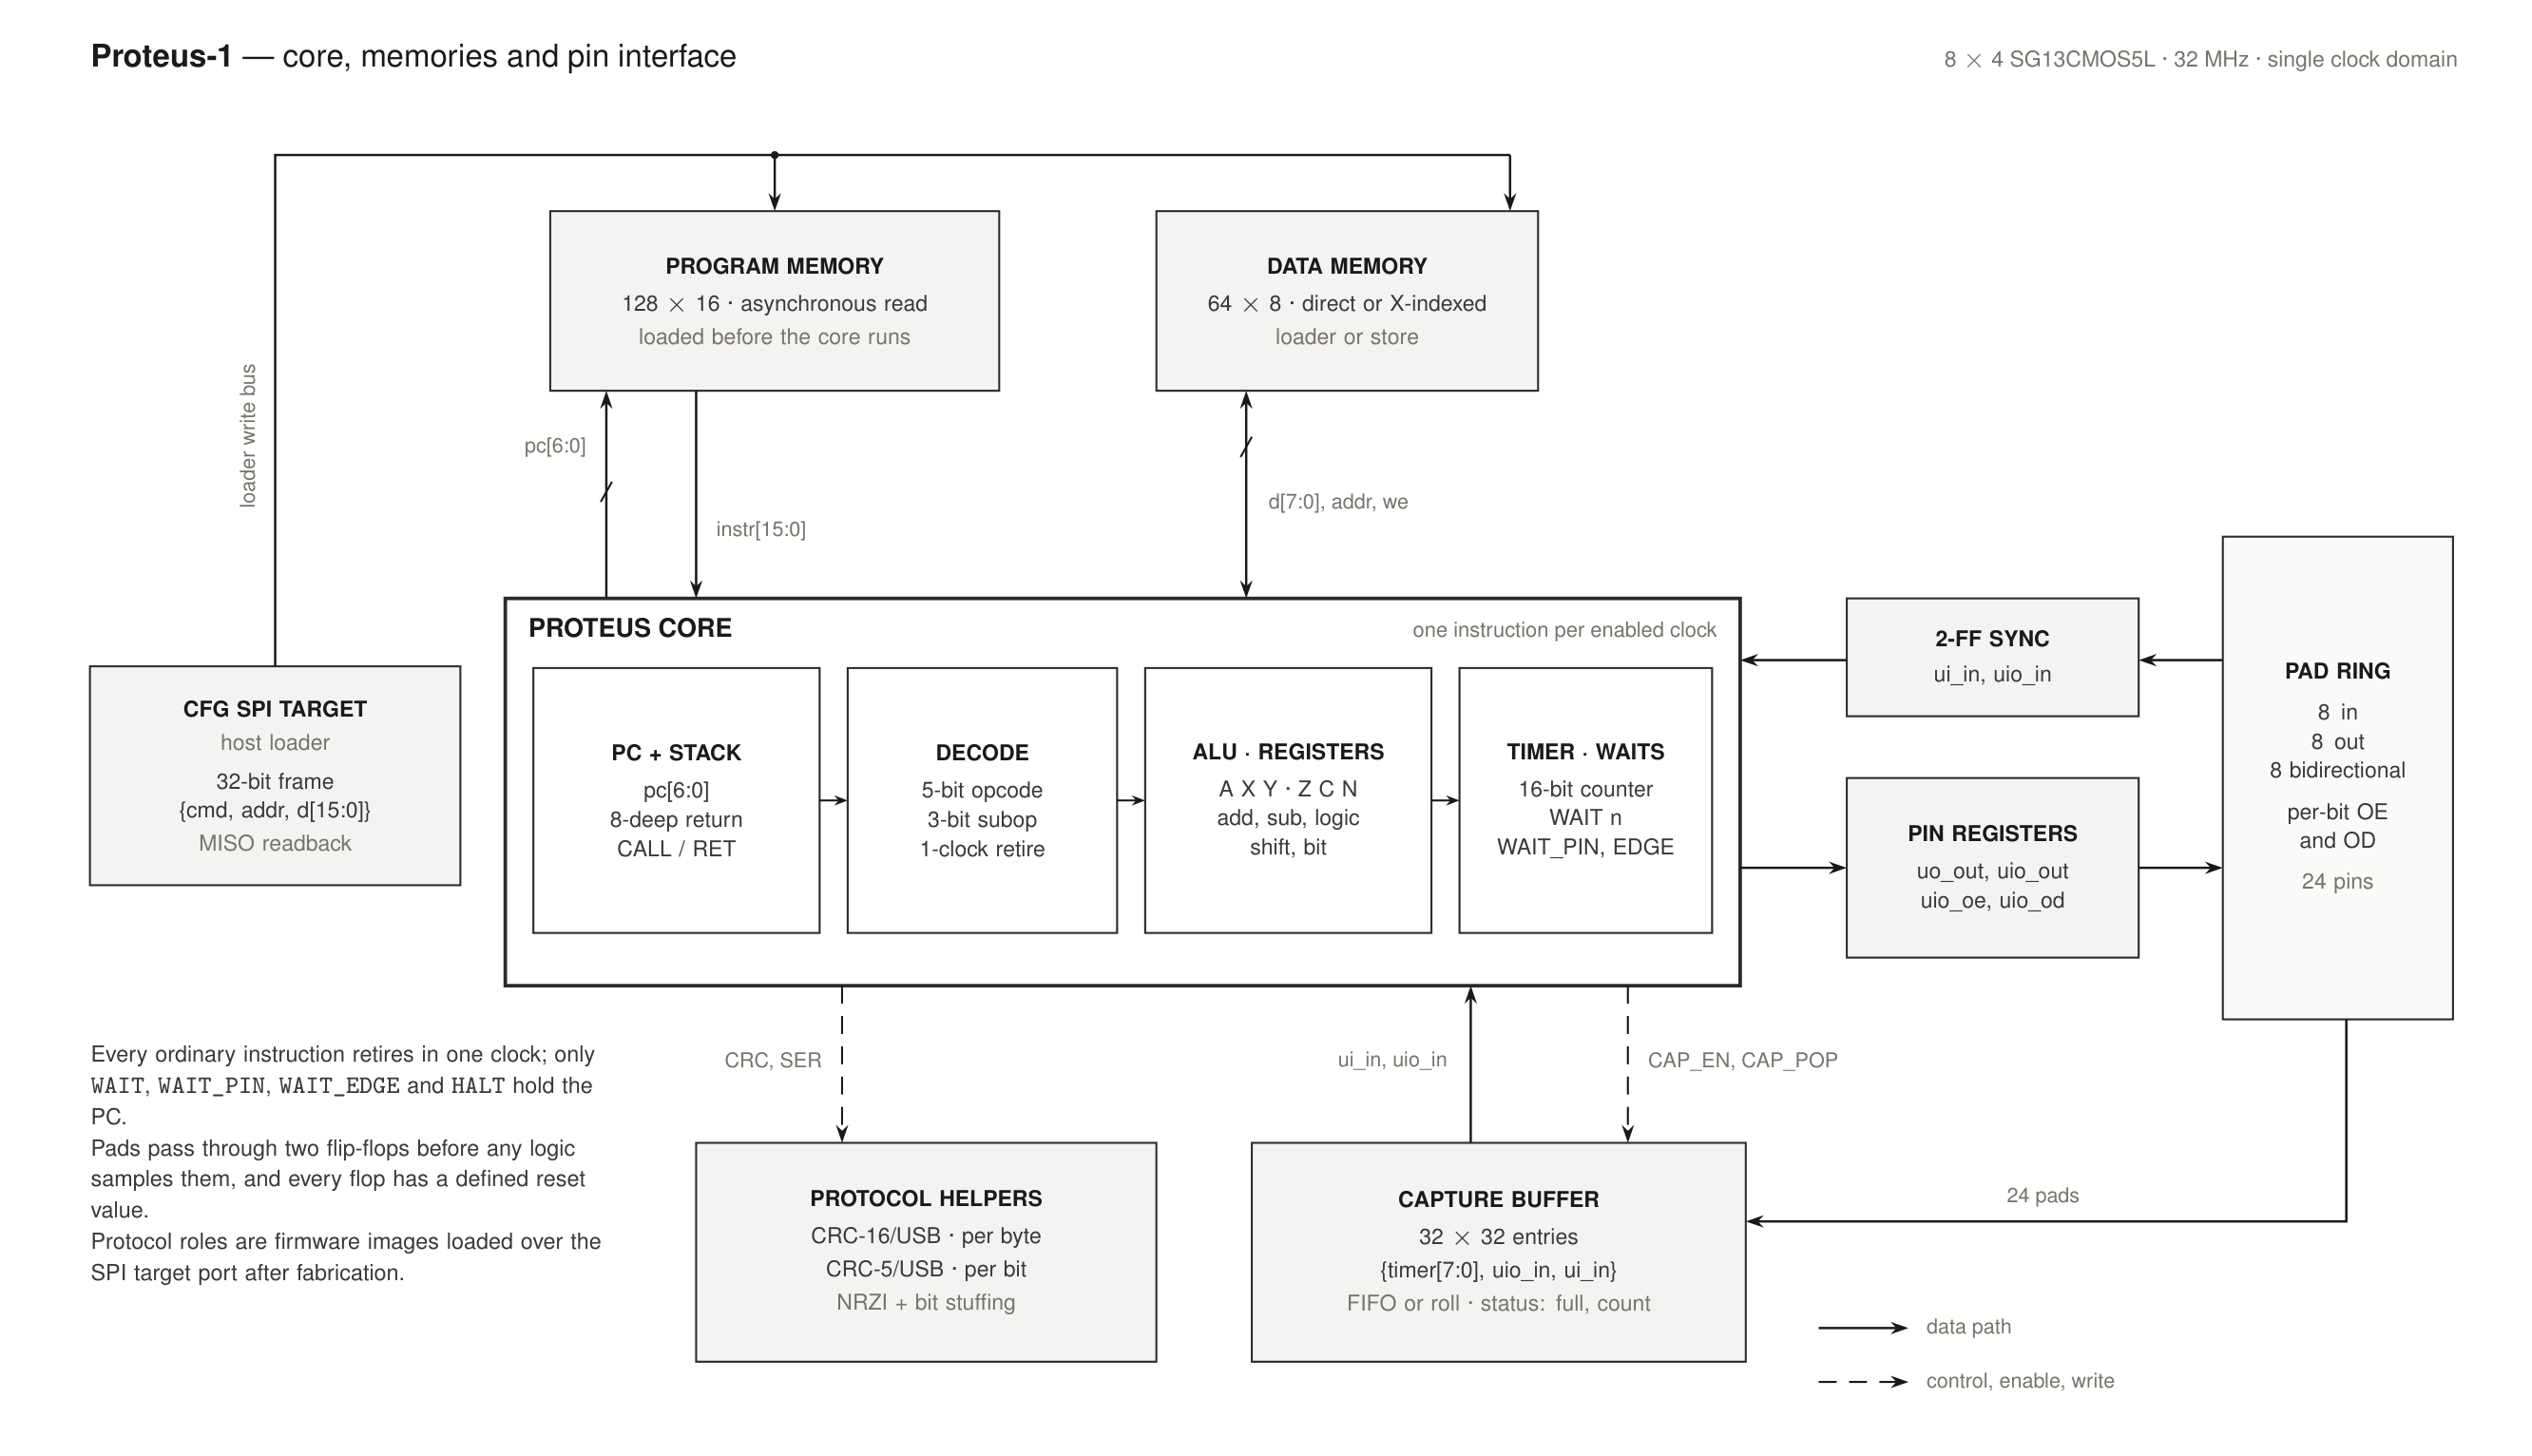
\includegraphics[width=0.94\linewidth]{images/block_diagram.png}
\caption{Block diagram: core, pin registers, capture engine, program memory and
host loader inside the 8 \(\times\) 4 pad ring.}
\end{figure}

% ------------------------------------------------------------------ section 2
\section{Features}

\begin{itemize}
  \item \textbf{8-bit accumulator CPU} --- \texttt{A}, \texttt{X}, \texttt{Y};
        7-bit \texttt{PC}; 8-deep circular return stack; \texttt{Z}/\texttt{C}/\texttt{N}
        flags. Fifteen opcode classes, one clock each.
  \item \textbf{128 \(\times\) 16 program memory} and \textbf{64 \(\times\) 8 data
        memory}, written by the host over the loader port.
  \item \textbf{24 digital pins} --- 8 dedicated inputs, 8 dedicated outputs, and
        8 bidirectional pins with per-bit output enable and per-bit open-drain
        mode, so I2C, wired-OR buses and shared pinouts need no external glue.
  \item \textbf{Exact delays} --- \texttt{WAIT} $n$ (1--255, $0$ = 256),
        \texttt{WAIT\_PIN0/1} on a pin mask, \texttt{WAIT\_EDGE} on any masked change.
  \item \textbf{16-bit cycle counter} with an atomic low/high read pair.
  \item \textbf{32-entry capture buffer} recording
        \{\texttt{cycle[7:0]}, \texttt{uio\_in}, \texttt{ui\_in}\} on every pin
        change, in drop-on-full FIFO mode or roll mode (newest 32 edges).
  \item \textbf{CRC helpers} --- CRC-16/USB, one byte per instruction, reproducing
        the published check value \texttt{0xB4C8} for \texttt{"123456789"};
        CRC-5/USB, one bit per instruction.
  \item \textbf{NRZI line coder with bit stuffing} and its matching
        \textbf{receiver with stuffing removal} and a sticky error latch, for
        low-speed USB framing.
  \item \textbf{Host loader} on \texttt{ui\_in[7:5]} with readback on
        \texttt{uo\_out[7]}, which returns to normal CPU output after configuration.
\end{itemize}

% ------------------------------------------------------------------ section 3
\section{Pin configuration}

All pins are digital. \texttt{clk}, \texttt{rst\_n} and \texttt{ena} come from the
carrier. Reset state is the pin state after \texttt{rst\_n} is released and before
a program is loaded.

\begin{center}
\rowcolors{2}{white}{gray!7}
\begin{tabularx}{\linewidth}{@{}L{0.13\linewidth}L{0.10\linewidth}L{0.26\linewidth}X@{}}
\toprule
\textbf{Pin} & \textbf{Reset} & \textbf{Run-mode function} & \textbf{Notes}\\
\midrule
\texttt{ui\_in[0]} & input & GPIO / \texttt{IN0} & firmware-defined\\
\texttt{ui\_in[1]} & input & GPIO / \texttt{IN1} & used by the capture demo\\
\texttt{ui\_in[2]} & input & GPIO / \texttt{IN2} & \\
\texttt{ui\_in[3]} & input & GPIO / \textbf{UART RX} & \texttt{uart\_rx.s}, 8N1\\
\texttt{ui\_in[4]} & input & GPIO / \textbf{JTAG TDO} & sampled by \texttt{jtag\_idcode.s}\\
\texttt{ui\_in[5]} & input & \textbf{\texttt{CFG\_MOSI}} while CS\_N low & GPIO after configuration\\
\texttt{ui\_in[6]} & input & \textbf{\texttt{CFG\_SCK}} while CS\_N low & GPIO after configuration\\
\texttt{ui\_in[7]} & input & \textbf{\texttt{CFG\_CS\_N}}, active low & low holds the CPU\\
\texttt{uo\_out[0:6]} & 0 & GPIO outputs & any protocol, any pin\\
\texttt{uo\_out[7]} & 0 & \textbf{\texttt{CFG\_MISO}} while CS\_N low & \textbf{UART TX} otherwise\\
\texttt{uio[0]} & Z & GPIO & SPI CS, PS/2 DATA, JTAG TCK\\
\texttt{uio[1]} & Z & GPIO & SPI MOSI, PS/2 CLK, JTAG TMS\\
\texttt{uio[2]} & Z & GPIO & SPI MISO, I2C SCL, JTAG TDI\\
\texttt{uio[3]} & Z & GPIO & SPI SCK, I2C SDA\\
\texttt{uio[4:7]} & Z & GPIO & free\\
\bottomrule
\end{tabularx}
\end{center}

\texttt{uio} pins power up with output enable off, so a carrier may drive them
before a program is loaded. \texttt{IN} always reads the actual pad, not the
output register, which is what makes an open-drain bus readable.

\textbf{Open-drain rule.} With \texttt{uio\_oe[i]} = 1 and \texttt{uio\_od[i]} = 1,
the pad drives 0 when \texttt{uio\_out[i]} = 0 and releases when
\texttt{uio\_out[i]} = 1. No per-bit direction swapping is required.

% ------------------------------------------------------------------ section 4
\section{Electrical characteristics}

These are post-route numbers from the hardened netlist, not measurements. The
shuttle carrier supplies the rails; the design adds no supply, analog or clock
requirement of its own. Consult the carrier pinout for rail voltages.

\subsection{Power}

\begin{center}
\begin{tabularx}{\linewidth}{@{}L{0.34\linewidth}L{0.30\linewidth}X@{}}
\toprule
\textbf{Parameter} & \textbf{Condition} & \textbf{Value}\\
\midrule
Total power, typical & \texttt{typ\_1p20V\_25C}, 32\,MHz & \textbf{8.71\,mW}\\
\quad internal & & 7.27\,mW\\
\quad switching & & 1.38\,mW\\
\quad leakage & & 0.05\,mW\\
\bottomrule
\end{tabularx}
\end{center}

Power scales with clock frequency and with how hard firmware drives the pins.
8.71\,mW is the placer/STA estimate at the declared clock, not a worst case.

\subsection{Area and die}

\begin{minipage}[c]{0.46\linewidth}
\rowcolors{2}{white}{gray!7}
\begin{tabular}{@{}lr@{}}
\toprule
\textbf{Parameter} & \textbf{Value}\\
\midrule
Die & 1,724.16 \(\times\) 710.64\,\um\\
Die area & 1,225,260\,\umsq\\
Core area & 1,208,170\,\umsq\\
Placed cells & 469,393\,\umsq\\
Utilisation & 38.9\,\%\\
Standard cells & 28,191\\
Sequential cells & 3,734\\
DRC / LVS / antenna & 0 / 0 / 0\\
\bottomrule
\end{tabular}
\end{minipage}\hfill
\begin{minipage}[c]{0.50\linewidth}
\centering
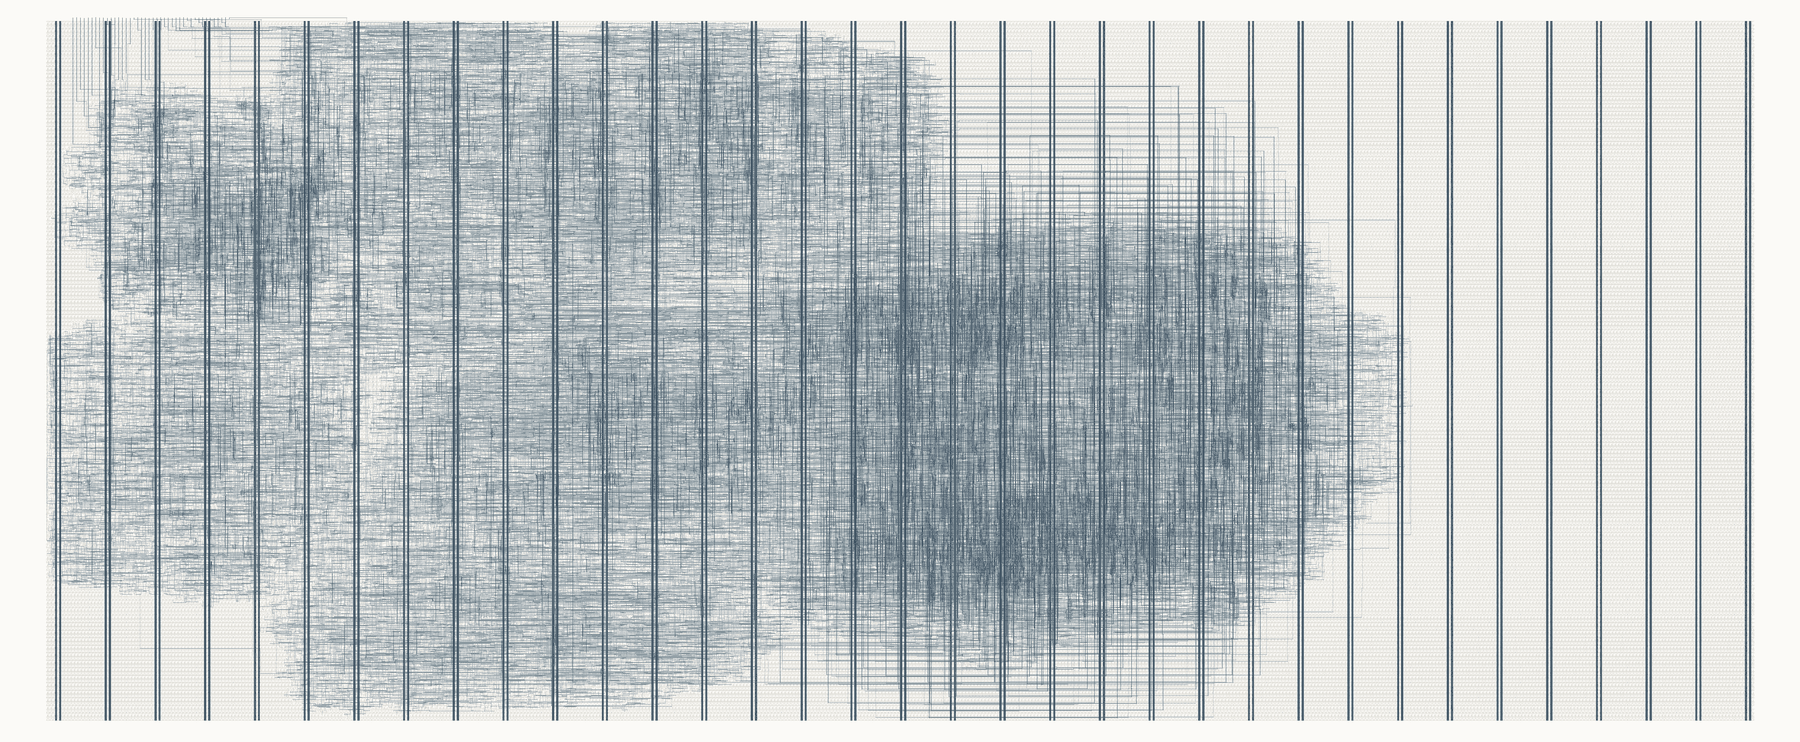
\includegraphics[width=\linewidth]{images/die.png}\\
{\footnotesize\itshape Layout rendered from the submitted GDS, 1.72 \(\times\) 0.71\,mm.}
\end{minipage}

% ------------------------------------------------------------------ section 5
\section{AC characteristics}

\begin{center}
\begin{tabularx}{0.94\linewidth}{@{}L{0.44\linewidth}L{0.18\linewidth}X@{}}
\toprule
\textbf{Parameter} & \textbf{Symbol} & \textbf{Value}\\
\midrule
Clock frequency & $f_{\mathrm{clk}}$ & \textbf{32\,MHz} maximum\\
Clock period & $t_{\mathrm{clk}}$ & 31.25\,ns\\
Setup slack, slow corner 1p08V/125\degC & & \textbf{+8.895\,ns}, 0 violators\\
Setup slack, typical 1p20V/25\degC & & +14.595\,ns, 0 violators\\
Setup slack, fast 1p32V/\(-40\)\degC & & +18.071\,ns, 0 violators\\
Hold slack, slow / typ / fast & & +0.654 / +0.313 / +0.108\,ns\\
Loader clock & $f_{\mathrm{SCK}}$ & $\le f_{\mathrm{clk}}/4$ = 8\,MHz\\
Reset pulse & $t_{\mathrm{rst}}$ & $\ge$ 1 clock, active low\\
\bottomrule
\end{tabularx}
\end{center}

There is no minimum clock frequency: a single clock domain with fully static
timing means the part runs down to DC. On an ECP5-25F FPGA the same RTL closes at
65.9\,MHz --- a portability check, not a silicon claim.

% ------------------------------------------------------------------ section 6
\needspace{10\baselineskip}
\section{Functional description}

\subsection{Memory and register map}

\begin{center}
\rowcolors{2}{white}{gray!7}
\begin{tabularx}{\linewidth}{@{}L{0.24\linewidth}L{0.16\linewidth}X@{}}
\toprule
\textbf{Resource} & \textbf{Size} & \textbf{Address / access}\\
\midrule
Program memory & 128 \(\times\) 16 & word \texttt{0x00}--\texttt{0x7F}; host-loaded, volatile\\
Data memory & 64 \(\times\) 8 & byte \texttt{0x00}--\texttt{0x3F} via \texttt{(X)} or \texttt{(imm)}\\
Return stack & 8 \(\times\) 8 & managed by \texttt{CALL}/\texttt{RET}; circular\\
Capture buffer & 32 \(\times\) 32 & \texttt{CAP\_POP}, then \texttt{CAP\_UI}/\texttt{UIO}/\texttt{TS}/\texttt{TSH}\\
Cycle counter & 16 & \texttt{TMR\_LO} latches the high byte, \texttt{TMR\_HI} reads it\\
CRC-16 / CRC-5 & 16 / 5 & reset to \texttt{0xFFFF} / \texttt{0x1F}\\
Identity & 8 & \texttt{ID} returns \texttt{0xA1}\\
\bottomrule
\end{tabularx}
\end{center}

Program memory is flip-flop based and undefined at power-up, so the part does
nothing useful until the host has loaded an image and set \texttt{run} = 1.

\needspace{12\baselineskip}
\subsection{Instruction set summary}

Sixteen bits per instruction: \texttt{opcode[15:11]}, \texttt{subop[10:8]},
\texttt{imm[7:0]}. \texttt{docs/isa.md} is normative; this is the index.

\begin{center}
\rowcolors{2}{white}{gray!7}
\begin{tabularx}{\linewidth}{@{}C{0.06\linewidth}L{0.12\linewidth}X@{}}
\toprule
\textbf{Op} & \textbf{Class} & \textbf{Covers}\\
\midrule
0 & \texttt{ALU} & \texttt{ADD ADC SUB SBC AND OR XOR CMP} with an immediate\\
1 & \texttt{SHIFT} & \texttt{SHL SHR ROL ROR ASR SWAP INC DEC} on \texttt{A}\\
2 & \texttt{LOAD} & immediates to \texttt{A/X/Y}, \texttt{LD}/\texttt{ST} via \texttt{X} or direct, \texttt{TFR}\\
3 & \texttt{IO} & \texttt{OUT} to \texttt{uo}/\texttt{uio}/OE/open-drain, \texttt{IN} from \texttt{ui}/\texttt{uio}\\
4 & \texttt{BRANCH} & \texttt{JMP JZ JNZ JC JNC CALL RET DJNZ}\\
5 & \texttt{TIME} & \texttt{WAIT}, \texttt{WAIT\_PIN0/1}, \texttt{WAIT\_EDGE}, \texttt{HALT}\\
6 & \texttt{BIT} & \texttt{SETB CLRB TGLB} on \texttt{uo}, \texttt{uio}, \texttt{uio\_oe}\\
7 & \texttt{MISC} & \texttt{NOP}, \texttt{INC/DEC} of \texttt{X}/\texttt{Y}, register aliases\\
8 & \texttt{ALUX} & the ALU table with \texttt{X} as the operand\\
9 & \texttt{ALUY} & the ALU table with \texttt{Y} as the operand\\
10 & \texttt{TIMER} & \texttt{TMR\_LO}, \texttt{TMR\_HI}, \texttt{TMR\_CLR}, \texttt{ID}\\
11 & \texttt{CAP} & \texttt{CAP\_EN} (FIFO/roll), \texttt{CAP\_POP}, \texttt{CAP\_UI}, \texttt{CAP\_UIO}, \texttt{CAP\_TS}, \texttt{CAP\_TSH}, \texttt{CAP\_STATUS}, \texttt{CAP\_CLR}\\
12 & \texttt{CRC} & \texttt{CRC16\_RST/ADD/LO/HI}, \texttt{CRC5\_RST/BIT}, \texttt{CRC5}\\
13 & \texttt{SER} & \texttt{SER\_LD}, \texttt{SER\_NEXT}, \texttt{SER\_LEVEL}, \texttt{SER\_BUSY}, \texttt{SER\_ONES}, \texttt{SER\_SET}, \texttt{SER\_JK}\\
14 & \texttt{RX} & \texttt{RX\_RST}, \texttt{RX\_BIT}, \texttt{RX\_ONES}, \texttt{RX\_ERR}\\
15--31 & reserved & execute as \texttt{NOP}; the assembler rejects them\\
\bottomrule
\end{tabularx}
\end{center}

\textbf{Cycle cost.} One clock for every instruction except \texttt{WAIT} $n$
(exactly $n$, $0$ = 256), \texttt{WAIT\_PIN*} and \texttt{WAIT\_EDGE} (at least
one, until the condition holds) and \texttt{HALT} (one, then stops until reset).

% ------------------------------------------------------------------ section 7
\section{Host loader interface}

An SPI mode-0 target on \texttt{ui\_in[7:5]}, with \texttt{uo\_out[7]} as MISO
while CS\_N is low. Frames are 32 bits, MSB first:

\begin{center}
\texttt{\{\,command[7:0], address[7:0], data[15:0]\,\}}
\end{center}

\begin{center}
\rowcolors{2}{white}{gray!7}
\begin{tabularx}{0.9\linewidth}{@{}C{0.14\linewidth}X@{}}
\toprule
\textbf{Command} & \textbf{Meaning}\\
\midrule
\texttt{0x00} & no operation; also the read-response frame\\
\texttt{0x01} & write program word: \texttt{prog[address[6:0]]} \(\leftarrow\) \texttt{data}\\
\texttt{0x02} & write data byte: \texttt{data[address[5:0]]} \(\leftarrow\) \texttt{data[7:0]}\\
\texttt{0x03} & control: \texttt{run} \(\leftarrow\) \texttt{data[0]}; \texttt{run} = 0 resets and holds the core\\
\texttt{0x04} & latch the program word at \texttt{address} for the next frame's MISO\\
\bottomrule
\end{tabularx}
\end{center}

Readback is pipelined: \texttt{0x04} latches a word and the \emph{next} frame
shifts it out during its first sixteen rising edges. Release the CPU with
\texttt{0x03} and \texttt{data} = 1. The reference host in \texttt{host/} runs at
100\,kHz, far below the 8\,MHz limit.

% ------------------------------------------------------------------ section 8
\needspace{17\baselineskip}
\section{Protocol capability matrix}

Rates are for the 32\,MHz clock and are set by firmware, not by fixed dividers.

\begin{center}
\rowcolors{2}{white}{gray!7}
\begin{tabularx}{\linewidth}{@{}L{0.19\linewidth}L{0.25\linewidth}L{0.17\linewidth}X@{}}
\toprule
\textbf{Role} & \textbf{Image} & \textbf{Rate} & \textbf{Limits}\\
\midrule
UART transmit & \texttt{uart\_tx.s} & 76.8\,kbaud 8N1 & TX on \texttt{uo\_out[7]}\\
UART receive & \texttt{uart\_rx.s} & 76.8\,kbaud 8N1 & samples \texttt{ui\_in[3]} mid-bit\\
SPI controller & \texttt{spi\_master.s}, \texttt{\_cpol1.s} & firmware-paced & modes 0--3 via two images\\
SPI target & \texttt{spi\_target.s} & firmware-paced & \textbf{mode 0 only}\\
I2C controller & \texttt{i2c\_master.s}, \texttt{\_400k.s} & 100\,kHz / 386\,kHz & external pull-ups\\
I2C target & \texttt{i2c\_target.s} & same two rates & address \texttt{0x28}\\
PS/2 device & \texttt{ps2\_device.s} & 10.5\,kHz & \textbf{transmit only}\\
JTAG master & \texttt{jtag\_idcode.s} & firmware-paced & reads IDCODE, \textbf{no IR scan}\\
USB framing & \texttt{usb\_data\_tx.s} & 21/22-clock dither & differential J/K, SE0, rate inside 1.5\,\%\\
Logic analyser & \texttt{capture\_demo.s} & every clock & 32 entries, FIFO or roll\\
\bottomrule
\end{tabularx}
\end{center}

% ------------------------------------------------------------------ section 9
\section{Errata and limitations}

\begin{enumerate}
  \item \textbf{No silicon.} Every number is from static timing, power and
        DRC/LVS on the hardened netlist. Nothing has been measured on a die.
  \item \textbf{Three classes of flow warning} at the slow corner: 41 max-slew
        and 2 max-cap reports, 293 max-fanout reports across corners, and one
        non-critical disconnected pin. None is a setup or hold violation; the
        flow error count is 0.
  \item \textbf{SPI target is mode 0 only.} The controller covers modes 0--3
        with two firmware images.
  \item \textbf{PS/2 is transmit-only.} A keyboard or host receiver is not
        implemented.
  \item \textbf{JTAG is a master that reads IDCODE} without an IR scan, valid
        because IEEE 1149.1 places IDCODE in the instruction register out of reset.
  \item \textbf{USB is line code and packet structure}, not a compliant PHY: the
        rate is dithered inside 1.5\,\% and SE0 is driven, but there is no
        transceiver, no board pull-up, and the eight bit slots assume a packet
        that needs no stuffed bit.
  \item \textbf{Program memory is volatile} and undefined at power-up; the host
        must load an image before \texttt{run} = 1.
  \item \textbf{Opcodes 15--31 are reserved} and execute as \texttt{NOP}. Firmware
        must not use them; the assembler refuses to emit them.
  \item \textbf{Formal verification is bounded} --- 40-cycle BMC plus temporal
        induction over six properties, not full ISA equivalence.
\end{enumerate}

% ----------------------------------------------------------------- section 10
\section{Related documents}

\begin{center}
\begin{tabularx}{0.94\linewidth}{@{}L{0.30\linewidth}X@{}}
\toprule
\textbf{Document} & \textbf{Contents}\\
\midrule
\texttt{docs/isa.md} & normative instruction set, encodings, flags, cycle counts\\
\texttt{docs/architecture.md} & blocks, area trade-offs, retime history\\
\texttt{docs/verification.md} & what each test proves, signoff numbers, gaps\\
\texttt{docs/info.md} & bring-up walkthrough and per-protocol hookup\\
\texttt{docs/competition.md} & design rationale and novelty\\
\texttt{docs/submission-checklist.md} & requirement-by-requirement evidence\\
\bottomrule
\end{tabularx}
\end{center}

Ordering: this part is not for sale. It is fabricated through the Tiny Tapeout
shuttle from this repository, and the RTL, tools, tests and documentation are
Apache-2.0.

% ----------------------------------------------------------------- section 11
\section{Revision history}

\begin{center}
\begin{tabularx}{\linewidth}{@{}C{0.12\linewidth}C{0.18\linewidth}X@{}}
\toprule
\textbf{Revision} & \textbf{Date} & \textbf{Basis}\\
\midrule
1.0 & 2026-11-17 & First datasheet; 8 \(\times\) 4 signoff from run \texttt{43957356626}, commit \texttt{18f08e0}\\
\bottomrule
\end{tabularx}
\end{center}

\end{document}
